% !TeX spellcheck = ru_RU
% !TEX root = vkr.tex

\section{Описание решения}


\subsection{Модуль с топологией RNN GRU}
\label{subsec:task1}


Основная идея данного модуля — предоставить возможность создания GRU-сети в рамках существующей архитектуры \texttt{DEGANN}. Для этого был разработан класс \texttt{TensorflowGRUNet}, который наследуется от \texttt{tf.keras.Model} и определяет необходимую логику построения слоёв GRU, их инициализацию, а также способ компоновки выходных данных. Важным моментом является то, что реализация идёт в связке с существующей инфраструктурой фреймворка \texttt{DEGANN}, где выбор конкретной топологии сети (в данном случае GRU) осуществляется через параметр \texttt{net\_type}, передаваемый при создании экземпляра класса \texttt{IModel}.

\subsubsection{Основные параметры и их назначение}
Класс \texttt{TensorflowGRUNet} включает несколько важных параметров, которые определяют архитектуру сети:
\begin{itemize}
    \item \textbf{input\_size:} размер входных данных. Задаёт количество входных признаков в данных.
    \item \textbf{block\_size:} список, определяющий количество нейронов в каждом слое GRU. Все слои должны иметь одинаковое количество нейронов.
    \item \textbf{output\_size:} количество выходных нейронов. Обычно для задач регрессии используется один выходной нейрон.
    \item \textbf{activation\_func и recurrent\_activation:} функции активации для основного состояния и рекуррентного состояния соответственно. По умолчанию используются \texttt{tanh} и \texttt{sigmoid}, так как они являются стандартными для GRU.
    \item \textbf{dropout\_rate:} уровень dropout, добавляемый после каждого слоя GRU для предотвращения переобучения.
    \item \textbf{weight и biases:} инициализаторы весов и смещений. Используются случайные значения в заданном диапазоне для начальной настройки параметров модели.
    \item \textbf{return\_sequences:} флаг, определяющий, будет ли сеть возвращать последовательности — это важно для многослойных рекуррентных сетей.
\end{itemize}

Данные параметры позволяют гибко настраивать модель под задачу, сохраняя при этом целостность и удобство использования в экосистеме \texttt{DEGANN}.

\subsubsection{Фрагмент инициализации параметров для GRU-топологии:}
Ниже мы приводим упрощённый фрагмент кода из реализации класса \texttt{TensorflowGRUNet}, в котором инициализируются вышеупомянутые параметры   :

\begin{lstlisting}[language=Python, breaklines, caption={Фрагмент инициализации параметров в \texttt{TensorflowGRUNet}}]
class TensorflowGRUNet(tf.keras.Model):
    def __init__(
            self,
            input_size: int = 2,
            block_size: List[int] = None,
            output_size: int = 10,
            activation_func: str = "tanh",
            recurrent_activation: str = "sigmoid",
            dropout_rate: float = 0.2,
            weight=keras.initializers.RandomUniform(minval=-1, maxval=1),
            biases=keras.initializers.RandomUniform(minval=-1, maxval=1),
            return_sequences: bool = False,
            **kwargs,
    ):
        super(TensorflowGRUNet, self).__init__(**kwargs)

        self.input_size = input_size
        self.count_size = block_size[0]
        self.gru_units = len(block_size)
        self.output_size = output_size
        self.activation_func = activation_func
        self.recurrent_activation = recurrent_activation
        self.dropout_rate = dropout_rate

        self.gru_layers = []  # list GRU layers
\end{lstlisting}

\subsubsection{Интеграция с \texttt{DEGANN}:}
Для внедрения новой архитектуры в \texttt{DEGANN} мы используем существующий интерфейс \texttt{IModel}. Создание модели осуществляется примерно следующим образом: при инициализации \texttt{IModel} мы передаем параметр \texttt{net\_type="GRUNet"}, что приводит к созданию внутри экземпляра класса сети с топологией \texttt{TensorflowGRUNet}.

Создание модели с топологией GRU происходит следующим образом:

\begin{lstlisting}[language=Python, caption=Создание модели с использованием топологии GRUNet]
count_size = 5  # количество слоёв
gru_units = 30  # количество нейронов в слое
shape = [gru_units] * count_size
GRU_IModel = IModel(
    input_size=1,
    output_size=1,
    net_type="GRUNet",  # указываем, что топология GRUNet
    block_size=shape)   # передаём размеры слоёв
\end{lstlisting}

В данном случае, внутри класса \texttt{IModel} вызывается метод \texttt{\_create\_functions["GRUNet"]}, возвращающий экземпляр \texttt{TensorflowGRUNet}, унаследованный от \texttt{tf.keras.Model}. Таким образом, мы сохраняем единообразный интерфейс для работы с моделями различных типов (DenseNet, GRUNet и т.д.) внутри \texttt{DEGANN}.

\begin{lstlisting}[language=Python, breaklines, caption=]
class IModel(object):
    def __init__(
        self,
        input_size: int,
        output_size: int,
        block_size: List[int] = None,
        activation_func="sigmoid",
        weight_init=tf.random_uniform_initializer(minval=-1, maxval=1),
        bias_init=tf.random_uniform_initializer(minval=-1, maxval=1),
        name="net",
        net_type="DenseNet",
        is_debug=False,
        **kwargs,
    ):
        self.network = _create_functions[net_type](
            input_size,
            block_size,
            activation_func=activation_func,
            weight=weight_init,
            biases=bias_init,
            output_size=output_size,
            is_debug=is_debug,
            **kwargs,
        )
        self._input_size = input_size
        self._output_size = output_size
        self._shape = block_size
        self._name = name
        self._is_debug = is_debug
        self.set_name(name)
        # остальная реализация IModel

_create_functions = defaultdict(lambda: TensorflowDenseNet)
_create_functions["DenseNet"] = TensorflowDenseNet
_create_functions["GRUNet"] = TensorflowGRUNet
\end{lstlisting}

\subsubsection{Как работает класс TensorflowGRUNet}
При инициализации класс \texttt{TensorflowGRUNet} создаёт несколько GRU-слоёв, каждый из которых имеет одинаковое количество нейронов, заданное параметром \texttt{block\_size}. На этапе инициализации происходит проверка, чтобы все слои сети имели одинаковый размер, поскольку это важное условие для корректной работы рекуррентных нейронных сетей. Если размер слоёв отличается, выбрасывается исключение.

\begin{lstlisting}[language=Python, breaklines, caption=Проверка размера слоев]
# checking |block_size| for data accuracy
if block_size is None or not all(size == block_size[0] for size in block_size):
    raise ValueError("\n//ERROR//\n"
        f"All layers in Recurrent Neural Networks must have the same number of neurons in each layer "
        f"\nReceived block_size: {block_size}")
\end{lstlisting}

Ключевая часть кода для создания слоёв выглядит следующим образом:

\begin{lstlisting}[language=Python, breaklines, caption=Инициализация GRU-слоёв]
for i in range(len(block_size)):
    self.gru_layers.append(
        keras.layers.GRU(
            units=block_size[0],
            activation=activation_func,
            recurrent_activation=recurrent_activation,
            return_sequences=True if i < len(block_size) - 1 else return_sequences,
            kernel_initializer=weight,
            bias_initializer=biases,
            name=f"GRULayer{i}"
        )
    )
    # Добавление dropout-слоя
    self.gru_layers.append(
        keras.layers.Dropout(rate=self.dropout_rate, name=f"DropoutLayer{i}")
    )
\end{lstlisting}

Здесь для каждого слоя создаётся GRU-слой с заданным количеством нейронов \texttt{block\_size[0]}, функциями активации, инициализаторами весов и смещений, а также параметром \texttt{return\_sequences}, который управляет, будет ли слой возвращать последовательности.

После каждого GRU-слоя добавляется слой Dropout для предотвращения переобучения. Эти слои помогают повысить устойчивость модели, добавляя случайные обнуления нейронов во время тренировки.

\subsubsection{Реализация функции call}
Функция \texttt{call} является важной частью класса \texttt{TensorflowGRUNet}, поскольку она выполняет прямой проход через сеть. В этой функции данные проходят через все GRU-слои, а затем через выходной полносвязный слой:

\begin{lstlisting}[language=Python, caption=Функция call]
def call(self, inputs, **kwargs):
    x = inputs
    for gru_layer in self.gru_layers:
        x = gru_layer(x, **kwargs)
    return self.out_layer(x, **kwargs)
\end{lstlisting}

Здесь переменная \texttt{x} передаётся через все GRU-слои, и после прохождения через последний слой, результат передаётся в выходной слой, который выполняет линейную активацию для задач регрессии.

\subsubsection{Особенности реализации}
Ключевой особенностью реализации является соблюдение совместимости с другими компонентами библиотеки DEGANN, что позволяет использовать стандартные методы обучения, тестирования и экспорта моделей. Например, параметры модели могут быть экспортированы в виде словаря, что упрощает сохранение и интеграцию в другие модули:

\begin{lstlisting}[language=Python, caption=Экспорт модели в словарь]
def to_dict(self):
    return {
        "net_type": "GRU",
        "input_size": self.input_size,
        "gru_units": self.gru_layers[0].units,
        "count_size": len(self.gru_layers) // 2,
        "output_size": self.output_size,
    }
\end{lstlisting}

Этот метод позволяет сохранить ключевые параметры модели, такие как тип сети, количество нейронов в слоях, количество слоёв и выходной размер, в виде словаря для дальнейшего использования или интеграции с другими частями системы.



\subsection{Датасет и сложно-аппроксимируемая функция}
\label{subsec:task2}

\subsubsection{Генерация датасета}
Для тестирования работы архитектуры GRU-сети был подготовлен специальный датасет, который генерировался с помощью встроенных инструментов библиотеки \texttt{DEGANN}. В качестве сложно-аппроксимируемой функции была выбрана функция \texttt{hardsin}, которая была добавлена в модуль \texttt{functions.py}:

\begin{lstlisting}[language=Python, breaklines, caption=Реализация функции \texttt{hardsin} в \texttt{functions.py}]
def hardsin(x):
    return np.sin(np.log(x**np.sin(10*x)))
hardsin = hardsin
\end{lstlisting}

Эта функция обладает сложной математической структурой, что делает её трудно аппроксимируемой стандартными архитектурами нейронных сетей. Её аналитическое выражение имеет следующий вид:

\[
f(x) = \sin\left(\ln(x^{\sin(10x)})\right)
\]

\subsubsection{График функции}
На рисунке ниже представлен график функции \texttt{hardsin}, демонстрирующий её сложное поведение:

\begin{figure}[H]
    \centering
    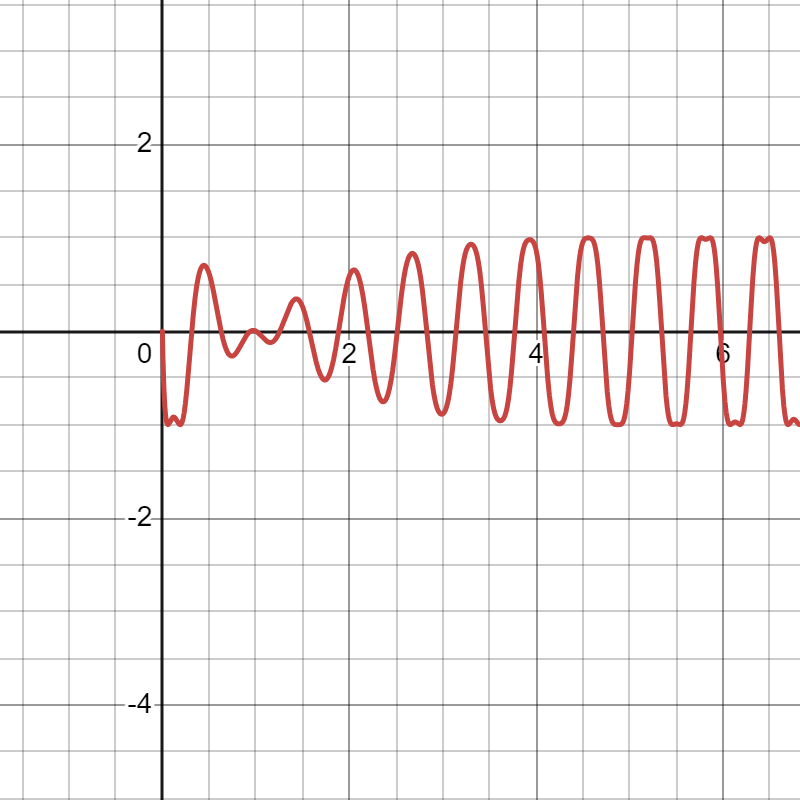
\includegraphics[width=0.8\textwidth]{figures/graph_hardsin.png}
    \caption{График функции $f(x) = \sin\left(\ln(x^{\sin(10x)})\right)$}
    \label{fig:hardsin_graph}
\end{figure}

\subsubsection{Загрузка и обработка данных}
Для создания тренировочного и валидационного наборов данных использовались встроенные методы генерации датасетов в \texttt{DEGANN}, которые позволяют сохранять данные в формате \texttt{.csv} для последующего использования. Пример кода загрузки данных:

\begin{lstlisting}[language=Python, breaklines, caption=Загрузка данных из CSV-файлов]
base_dir = os.path.dirname(__file__)
name_dataset = "hardsin_1000"

csv_path = os.path.join(base_dir, "../../experiments/data/" + name_dataset + "_train.csv")
val_csv_path = os.path.join(base_dir, "../../experiments/data/" + name_dataset + "_validate.csv")

train_data = pd.read_csv(csv_path, names=["x", "y"])
val_data = pd.read_csv(val_csv_path, names=["x", "y"])

train_data_x = train_data["x"].values.reshape(-1, 1)
train_data_y = train_data["y"].values.reshape(-1, 1)
val_data_x = val_data["x"].values.reshape(-1, 1)
val_data_y = val_data["y"].values.reshape(-1, 1)
\end{lstlisting}

\subsubsection{Добавление шума}

Для повышения устойчивости модели и её способности к обобщению в процессе обучения на тренировочные данные добавлялся шум, который следовал нормальному распределению. Это позволяет модели лучше адаптироваться к реальным данным, которые часто содержат случайные колебания и погрешности. Нормальное распределение (также называемое гауссовским распределением) является одним из наиболее часто используемых видов распределений в статистике и машинном обучении.

\paragraph{Формула нормального распределения:}
Нормальное распределение определяется следующей плотностью вероятности:

\[
f(x) = \frac{1}{\sqrt{2 \pi \sigma^2}} e^{-\frac{(x - \mu)^2}{2 \sigma^2}}
\]

где:
\begin{itemize}
    \item $\mu$ --- математическое ожидание (среднее значение),
    \item $\sigma$ --- стандартное отклонение (мера разброса данных),
    \item $x$ --- случайная величина.
\end{itemize}

Параметры $\mu$ и $\sigma$ в нашем случае были рассчитаны на основе целевой переменной тренировочного датасета $\texttt{train\_data\_y}$, чтобы шум соответствовал масштабу данных.

\paragraph{Применение шума в датасете:}
Добавление шума выполнялось с использованием библиотеки NumPy, где функция \texttt{np.random.normal()} генерирует массив случайных значений, следующих нормальному распределению. В нашем случае среднее значение шума $\mu = 0$, а стандартное отклонение рассчитывается как $0.1 \cdot \sigma$, где $\sigma$ --- стандартное отклонение значений целевой переменной. Формула добавления шума выглядит следующим образом:

\[
\texttt{train\_data\_y\_noisy} = \texttt{train\_data\_y} + \xi, \quad \xi \sim \mathcal{N}(0, 0.1 \cdot \sigma)
\]

\paragraph{Реализация в коде:}
Ниже приведён код, демонстрирующий, как добавляется шум с нормальным распределением к целевой переменной тренировочного датасета:

\begin{lstlisting}[language=Python, breaklines, caption=Добавление шума с нормальным распределением]
import numpy as np
# Рассчитываем  стандартное  отклонение  данных
sigma = np.std(train_data_y)
# Генерируем  шум  с  нормальным  распределением
noise = np.random.normal(0, sigma * 0.1, train_data_y.shape)
# Добавляем  шум  к  целевой  переменной
train_data_y_noisy = train_data_y + noise
\end{lstlisting}
Этот подход позволяет модели лучше обобщать данные, избегая переобучения на исходный датасет.

\subsubsection{Временные последовательности}
Рекуррентные нейронные сети, такие как GRU, предназначены для обработки временных последовательностей. Их ключевая особенность заключается в возможности сохранять информацию о предыдущих состояниях для анализа текущих данных. Это делает их идеальными для задач, где данные зависят от контекста, например, аппроксимация временных рядов.

Для корректной работы RNN данные из исходного датасета были преобразованы в последовательности фиксированной длины с помощью функции \texttt{create sequences}:

\begin{lstlisting}[language=Python, breaklines, caption=Создание временных последовательностей]
def create_sequences(data_x, data_y, time_steps):
    x, y = [], []
    for i in range(len(data_x) - time_steps):
        x.append(data_x[i:i + time_steps])
        y.append(data_y[i + time_steps])
    return np.array(x), np.array(y)

time_steps = 10
train_data_x, train_data_y = create_sequences(train_data_x, train_data_y, time_steps)
val_data_x, val_data_y = create_sequences(val_data_x, val_data_y, time_steps)
\end{lstlisting}

В данном примере \texttt{time\_steps} задаёт количество шагов в последовательности. Это означает, что каждый входной элемент сети состоит из \texttt{time\_steps} предыдущих значений, а целевая переменная соответствует следующему значению функции.

\paragraph{Почему RNN работают с временными последовательностями?}
Основное преимущество RNN заключается в их способности передавать информацию через скрытые состояния (\textit{hidden states}). В отличие от обычных нейронных сетей, которые обрабатывают каждый вход независимо, RNN сохраняют информацию из предыдущих шагов и используют её для обработки текущего ввода. Это реализуется через рекуррентную связь, которая обновляет скрытое состояние на каждом временном шаге:

\[
h_t = f(W_{xh} \cdot x_t + W_{hh} \cdot h_{t-1} + b_h),
\]

где:
\begin{itemize}
    \item $h_t$ --- скрытое состояние на шаге $t$,
    \item $x_t$ --- входные данные на шаге $t$,
    \item $W_{xh}$ и $W_{hh}$ --- весовые матрицы для входа и скрытого состояния соответственно,
    \item $b_h$ --- вектор смещения,
    \item $f$ --- нелинейная функция активации, например, $\tanh$.
\end{itemize}

Таким образом, скрытое состояние $h_t$ содержит информацию как о текущем входе $x_t$, так и о предыдущих состояниях $h_{t-1}$. Это позволяет сети «запоминать» ключевые элементы данных, важные для предсказания, что особенно полезно для задач, где контекст играет важную роль.

\paragraph{Важность временных последовательностей для GRU}
Архитектура GRU (Gated Recurrent Unit) улучшает традиционные RNN за счёт использования механизмов управления потоками информации, таких как:
\begin{itemize}
    \item \textit{update gate}, который определяет, сколько информации из предыдущего состояния следует сохранить
    \item \textit{reset gate}, позволяющий управлять степенью игнорирования информации из предыдущего состояния
    \item Итоговое скрытое состояние вычисляется как взвешенная комбинация текущего состояния и нового кандидата состояния, где новое состояние зависит от текущего ввода и скрытого состояния
\end{itemize}

Эти механизмы позволяют GRU эффективно работать с временными последовательностями, игнорируя неважную информацию и выделяя ключевые зависимости в данных. Благодаря этому, временные последовательности, преобразованные в фиксированные окна, позволяют RNN, в частности GRU, обучаться на задачах, где данные имеют явные временные или причинно-следственные зависимости.


\subsection{Создание модели и реализация callback-функций}
\label{subsec:task3}

В процессе разработки и обучения модели важно не только корректно настроить её архитектуру, но и обеспечить инструментами, позволяющими наглядно оценивать ход обучения, качество модели и её производительность. Это включает как отслеживание ключевых метрик, таких как функция потерь, так и визуализацию предсказаний модели на различных этапах.

Основные цели анализа обучения и валидации включают:
\begin{itemize}
    \item \textbf{Оценка функции потерь}: Анализ функции потерь на тренировочных и валидационных данных позволяет выявить динамику обучения, а также возможные проблемы, такие как переобучение или недостаточное обучение.
    \item \textbf{Раннее прекращение обучения}: Обеспечивает остановку обучения, если модель перестала улучшаться, предотвращая ненужные вычисления и переобучение.
    \item \textbf{Сохранение лучшей модели}: Позволяет фиксировать параметры модели с минимальной валидационной ошибкой, чтобы использовать её для дальнейших экспериментов.
    \item \textbf{Визуализация}: Сравнение предсказаний модели с истинной функцией и визуализация потерь предоставляет интуитивное понимание, насколько хорошо модель аппроксимирует данные.
    \item \textbf{Измерение времени обучения}: Позволяет оценить, насколько эффективно используются вычислительные ресурсы при обучении модели.
\end{itemize}

Для достижения этих целей были реализованы и интегрированы несколько callback-функций, обеспечивающих автоматическое выполнение перечисленных выше задач. Эти callback-функции разработаны как часть архитектуры проекта DEGANN и могут быть легко добавлены при обучении любой модели.

\subsubsection{Создание модели GRU}
Для создания модели с использованием топологии GRU использовалась модульная архитектура DEGANN, наследуемую от базового класса \texttt{IModel}, не внося изменений в его структуру. Такой подход позволил адаптировать сеть GRU к задачам аппроксимации дифференциальных уравнений и интегрировать её в существующий функционал проекта.

\subsubsection{Пример использования callback-функций}

Для анализа и визуализации обучения были разработаны и внедрены следующие callback-классы:
\begin{itemize}
    \item \texttt{LossTracking}: Отслеживает и сохраняет значения функции потерь на тренировочных и валидационных данных.
    \item \texttt{EarlyStopping}: Реализует раннее прекращение обучения при отсутствии улучшений в течение заданного количества эпох.
    \item \texttt{SaveBestModel}: Сохраняет параметры модели с минимальной валидационной ошибкой.
    \item \texttt{VisualizationTS}: Визуализирует процесс обучения и предсказания модели, сравнивая их с истинной функцией.
\end{itemize}

Ниже приведён пример использования данных callback-функций в процессе обучения модели GRU:

\begin{lstlisting}[language=Python, breaklines, caption=Пример настройки и использования callback-функций]
from degann.networks.callbacks import MeasureTrainTime, LossTracking, EarlyStopping, SaveBestModel, VisualizationTS

loss_before_train = GRU_IModel.evaluate(train_data_x, train_data_y, verbose=0)
val_loss_before_train = GRU_IModel.evaluate(val_data_x, val_data_y, verbose=0)

MeasureTrainTime = MeasureTrainTime()
Loss_tracking = LossTracking()
Early_stopping = EarlyStopping(patience=100)  # "patience" - the number of epochs without improvement
Save_best_model = SaveBestModel(GRU_IModel)
Visualization = VisualizationTS(train_data_x, train_data_y, val_data_x, val_data_y, name_dataset.split('_')[0], funcs)

GRU_IModel.train(train_data_x, train_data_y, validation_data=(val_data_x, val_data_y), epochs=epochs, verbose=0, callbacks=[MeasureTrainTime, Loss_tracking, Early_stopping, Save_best_model, Visualization])

loss_after_train = GRU_IModel.evaluate(train_data_x, train_data_y, verbose=0)
val_loss_after_train = GRU_IModel.evaluate(val_data_x, val_data_y, verbose=0)
\end{lstlisting}

\begin{lstlisting}[language=Tex, breaklines, caption=Пример получения данных от callback-функций]
Epoch 1: finished in: 6.68 seconds | Training Loss: 0.4940, Validation Loss: 0.4203
Epoch 2: finished in: 0.97 seconds | Training Loss: 0.4340, Validation Loss: 0.4031
Epoch 3: finished in: 1.05 seconds | Training Loss: 0.3875, Validation Loss: 0.3818
Epoch 4: finished in: 1.08 seconds | Training Loss: 0.3203, Validation Loss: 0.2576
Epoch 5: finished in: 1.09 seconds | Training Loss: 0.2171, Validation Loss: 0.1123
...
Epoch 49: finished in: 0.40 seconds | Training Loss: 0.0597, Validation Loss: 0.0272
Epoch 50: finished in: 0.48 seconds | Training Loss: 0.0617, Validation Loss: 0.0411
Total training time: 55.3523 seconds
Average time per epoch: 1.107045 seconds
Loss before training = 0.606187
Loss after training = 0.059869
different between Losses =0.546318
validation loss before training = 0.610131
validation loss after training = 0.041137
Difference in validation loss = 0.568993
\end{lstlisting}

\subsubsection{Описание callback-функций}

\textbf{LossTracking}: Позволяет отслеживать значения функции потерь на тренировочных и валидационных данных на каждой эпохе.

\textbf{EarlyStopping}: Реализует механизм ранней остановки обучения, если валидационная ошибка не уменьшается в течение заданного числа эпох \textbf{patience}. Это помогает избежать переобучения и экономит ресурсы.

\textbf{SaveBestModel}: Сохраняет лучшую модель, найденную в процессе обучения, фиксируя параметры сети с минимальной валидационной ошибкой.

\textbf{VisualizationTS}: Генерирует графики, отображающие:
\begin{itemize}
    \item Динамику функции потерь на тренировочных и валидационных данных.
    \item Сравнение истинной функции, предсказаний модели и тренировочных данных.
\end{itemize}

Данные callback-функции позволяют автоматизировать рутинные задачи анализа и визуализации обучения, делая процесс более удобным и наглядным.

\subsection{Метрика и гиперпараметры}
\label{subsec:task4}

Для эффективного обучения модели на основе архитектуры GRU необходимо тщательно подбирать как функцию потерь, так и параметры модели. В данном разделе представлены обоснования выбора ключевых компонентов, включая функцию потерь, оптимизатор, количество слоев и нейронов в каждом слое, а также влияние гиперпараметров на производительность модели.

\subsubsection{Функция потерь}

В качестве функции потерь для обучения модели была выбрана среднеквадратичная ошибка (\textit{Mean Squared Error}, MSE). Эта функция вычисляется по формуле:
\[
\text{MSE} = \frac{1}{n} \sum_{i=1}^{n} (y_i - \hat{y}_i)^2,
\]
где \( y_i \) — истинное значение, \( \hat{y}_i \) — предсказанное моделью значение, \( n \) — количество наблюдений.

Среднеквадратичная ошибка (MSE) была выбрана, поскольку задача аппроксимации функций и решения дифференциальных уравнений относится к классу задач регрессии. MSE является стандартным выбором для подобных задач из-за следующих причин:
\begin{itemize}
    \item MSE минимизирует квадраты ошибок, что позволяет существенно штрафовать крупные отклонения между предсказанными и истинными значениями. В задачах регрессии это помогает получить точные предсказания на всём диапазоне данных, что критически важно для задач аппроксимации сложных функций.
    \item Как показано в исследованиях \cite{Goodfellow} (Глава 5. Задачи регрессии и выбор функции потерь), MSE демонстрирует высокую эффективность в задачах регрессии, так как она позволяет моделям учитывать среднеквадратичное отклонение между предсказанными значениями и реальными метками. Это способствует устойчивой сходимости и снижению ошибки.
    \item MSE обладает хорошей интерпретируемостью и простотой вычисления, что делает её предпочтительным выбором как для небольших, так и для сложных моделей машинного обучения [2]. Она позволяет измерять общую степень расхождения между моделью и данными, обеспечивая ясное понимание качества обучения.
    \item В ходе собственных экспериментов было замечено, что MSE демонстрирует устойчивую сходимость модели на тренировочных данных, обеспечивая баланс между точностью предсказания и эффективностью обучения.
\end{itemize}

Таким образом, выбор MSE обусловлен её популярностью и доказанной эффективностью для задач регрессии, а также её способностью оптимизировать поведение модели на аппроксимируемых функциях.

\paragraph{Примечания.}
\begin{enumerate}
    \item Goodfellow, I., Bengio, Y., Courville, A. \textit{Deep Learning}. MIT Press, 2016. Глава 5. Задачи регрессии и выбор функции потерь.
    \item Géron, A. \textit{Hands-On Machine Learning with Scikit-Learn, Keras, and TensorFlow}. O'Reilly Media, 2019. Глава 4. Анализ методов регрессии и MSE.
\end{enumerate}


\subsubsection{Гиперпараметры модели}

Для архитектуры GRU важно выбирать параметры, обеспечивающие баланс между сложностью модели и доступными вычислительными ресурсами. После серии экспериментов оптимальными гиперпараметрами для модели были установлены следующие значения:
\begin{itemize}
    \item \textbf{Количество слоев}: \( \texttt{count\_size} = 5 \);
    \item \textbf{Количество нейронов в каждом слое}: \( \texttt{gru\_units} = 30 \);
    \item \textbf{Топология сети}: \( \texttt{shape} = [\texttt{gru\_units}] \times \texttt{count\_size} = [30, 30, 30, 30, 30] \).
\end{itemize}

Эти параметры были выбраны на основе следующих факторов:
\begin{itemize}
    \item Увеличение количества слоев или количества нейронов в слоях приводит к значительному росту количества параметров модели. Это, в свою очередь, требует больше вычислительных ресурсов и времени на обучение. Однако моих вычислительных мощностей недостаточно для работы с сильно усложненными моделями.
    \item Слишком маленькие параметры приводят к недообучению модели, особенно на сложных задачах аппроксимации функций. Оптимальные параметры (\( 5 \) слоев и \( 30 \) нейронов) позволили достичь хорошего компромисса между качеством модели и временем обучения.
    \item Выбранная топология (\( [30, 30, 30, 30, 30] \)) обеспечивает достаточную мощность модели для работы с временными последовательностями, не вызывая переобучения при разумном количестве эпох.
\end{itemize}

\subsubsection{Оптимизатор}

Для обучения модели был выбран оптимизатор \textit{Adam}, который зарекомендовал себя как один из наиболее эффективных методов оптимизации градиентного спуска. \textit{Adam} комбинирует преимущества методов \textit{Momentum} и \textit{RMSprop}, автоматически регулируя скорость обучения для каждого параметра. Это особенно полезно для рекуррентных сетей, которые могут страдать от проблемы затухающих или взрывающих градиентов.

Оптимизатор \textit{Adam} был выбран по следующим причинам:
\begin{itemize}
    \item Автоматическая настройка шага обучения ускоряет сходимость модели.
    \item Эффективность на задачах регрессии и работы с последовательностями.
    \item В экспериментах с архитектурой GRU оптимизатор показал стабильную сходимость.
\end{itemize}

\subsubsection{Влияние гиперпараметров на производительность}

Увеличение количества слоев и нейронов позволяет повысить выразительную способность модели, но при этом модель становится склонной к переобучению и требует значительно больше эпох для достижения хорошей сходимости. Однако из-за ограничений вычислительных мощностей количество слоев и нейронов было выбрано таким образом, чтобы достичь разумного баланса между сложностью модели и временем обучения.

Таким образом, выбор MSE в качестве функции потерь, оптимизатора \textit{Adam} и оптимальных гиперпараметров модели позволил создать эффективную архитектуру для аппроксимации дифференциальных уравнений, несмотря на ограниченные вычислительные ресурсы.